\documentclass[a4paper,10pt]{article}
\usepackage[utf8x]{inputenc}
\usepackage{amsmath}
\usepackage[margin=1.25in]{geometry}
\usepackage{algorithm}
\usepackage{algorithmic}
\usepackage{color}
\usepackage{epsfig}
\usepackage{multirow}
\usepackage[pdftex,colorlinks=true,urlcolor=blue,pdfstartview=FitH]{hyperref}
\DeclareGraphicsExtensions{.pdf,.pdftex_t,.png,.jpg}  % car pdflatex ne sait pas inclure de .eps
\pdfcompresslevel=9

\DeclareGraphicsExtensions{.pdf,.pdftex_t,.png,.jpg}  % car pdflatex ne sait pas inclure de .eps
\graphicspath{{./Figures/}{.}}

\usepackage{tikz}

\usepackage{verbatim}
\usetikzlibrary{arrows,shapes}

%opening
\title{Colored ants for solving dynamic job shop scheduling problem : application to a straddle carriers container terminal
% the straddle carriers container terminal test case
%Straddle carriers container terminal optimization : an ant colony based approach
%An ant colony based algorithm to solve job shop scheduling problem : application to a straddle carriers container terminal???
}
\author{Ga\"{e}tan~Lesauvage\thanks{~Corresponding author}, Stefan~Balev, Fr\'{e}d\'{e}ric~Guinand\\\\
\medskip
Universit\'{e} du Havre, LITIS EA 4108\\
BP 540, 76058 Le Havre, France\\
\medskip
E-mail: \{gaetan.lesauvage,stefan.balev,frederic.guinand\}@litislab.eu\\
\medskip
Phone: 0033 232 744 543
}


\begin{document}

\maketitle

\begin{abstract}
%Container terminal and JSSP
We present in this paper a real world application of a dynamic job shop scheduling problem: the straddle carriers missions scheduling problem. Indeed, in a straddle carriers container terminal, a mission consist in picking up a container from a location and then deliverying it to another one. Those operations must occured within given time windows to ensure the quality of service. Straddle carriers are very expensive equipment and their use must be optimized. The optimization objective is so to minimize the distance covered by the straddle carriers to execute the missions and in the meantime to minimize the overspent time windows.
%Dynamics
However the terminal is subject to many dynamic events such as the arrival of unexpected missions, the update of the time windows, or the straddle carriers failures for instance. The problem is then characterized as dynamic.
%ACO
We propose an ant colony based algorithm using a dynamic graph to provide near optimal solutions in low computation time.

\end{abstract}

%=============================================================================
\section{Introduction}
%=============================================================================

%Contexte => Développement du transport conteneurisé
With the development of trade activities which have continually increased, container has become the first mode of packaging for exchanging goods. Container terminals have been created all around the world in order to facilitate the transfer between ships and trucks or trains. The performance of these transfers has to be considered to reduce the waiting cost of the container terminal customers.

Le Havre’s harbor is the biggest harbor of France in container traffic. It is located at the North West cost of France, beside the Channel, sea door between the Atlantic and the North Sea. To keep competitive, the harbor has to provide a high quality of service and unceasingly develop new technologies and processes.

%Environnement => Terminal à conteneur : définitions des termes relatifs au conteneurs et à leur transport
Straddle carriers are used within the terminal to move containers. Those vehicles can lift a container from above and are very useful to move containers in the yard by driving over the lanes. They are also used to load or unload trucks or trains. Some of them are able to dynamically adapt the spreader size to any container dimensions while some of them require to be set up in the depot.%Cout unitaire extremement eleve + Conso fuel enorme => 


\begin{figure}[h]
  \begin{center}
  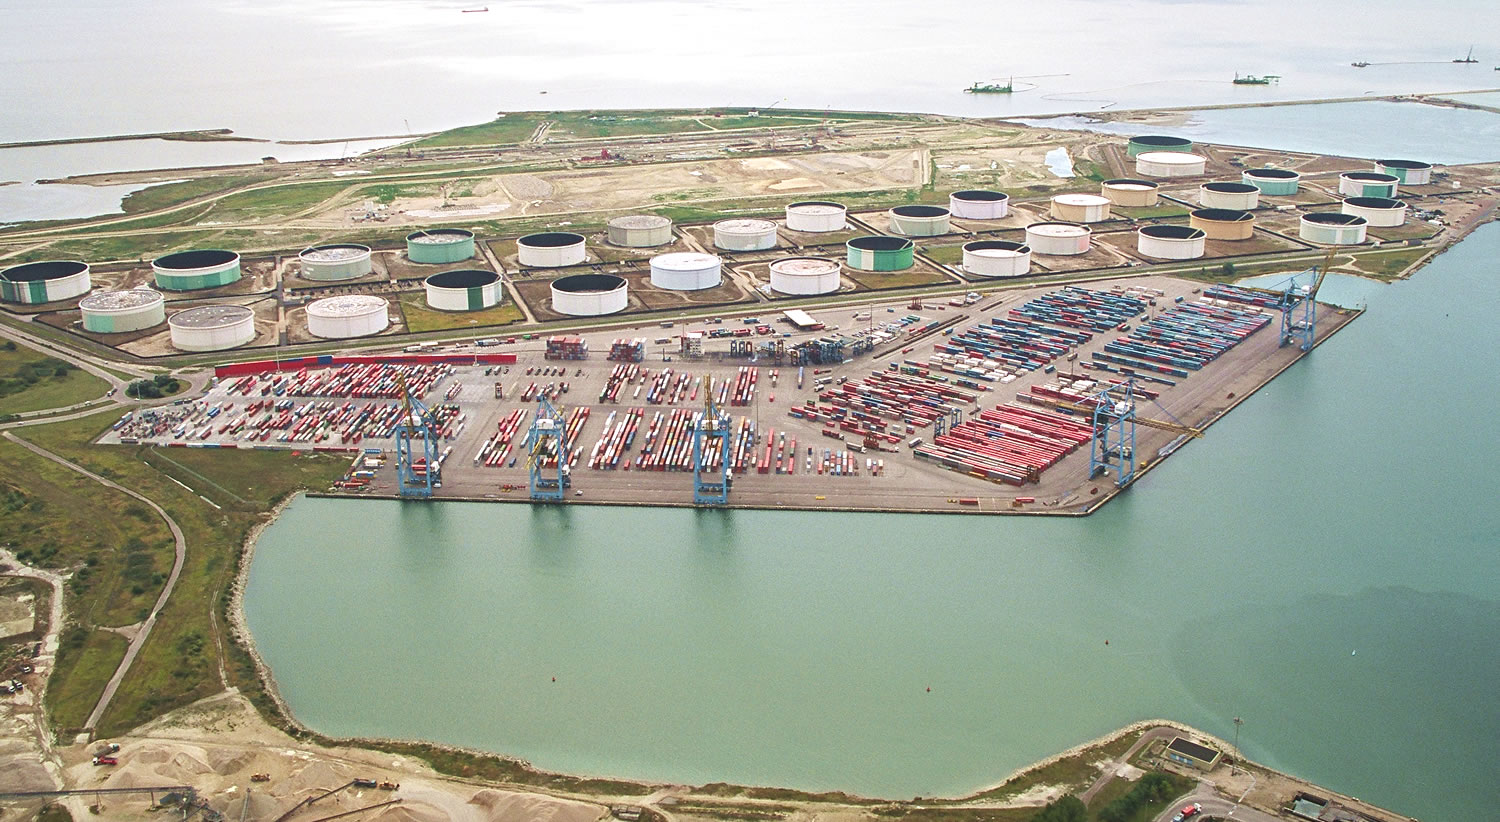
\includegraphics[width=0.6\textwidth]{Figures/terminalOfNormandy}
  \caption{The Terminal of Normandy, Le Havre's harbor, France.}
\end{center}
\end{figure}

Each move of a container by a straddle carrier can be seen like a mission. There are four kinds of missions :
\begin{itemize}
	\item Incoming container missions;
	\item Outgoing container missions;
	\item Transshipment missions;
	\item Staying container missions.
\end{itemize}

The first category concerns trucks, trains and ships unloading. Straddle carriers drive to the pick-up locations and unload the vehicles, and then lift the container, drive to the yard to stock it. Concerning ships, they are unloaded by quay cranes which stack the containers on the quay. Then, straddle carriers come to pick-up the containers.
The second category concerns trucks, trains and ships loading. In this case, straddle carriers start by picking-up a container from the yard and then drive to the delivery location (trucks areas, trains area or ship areas) to deliver it to their recipient. 
The third category of missions concerns the move of a container from a ship to another one.
Finally, the last kind of missions concerns internal yard optimization process. Indeed, in some cases, it can be useful to reorganize a part of the stock area in order to reduce further delivery times or to free strategic container slots for next unloading missions.

Two time windows are affected to every mission. One concerns the pickup phase, the other one is related to the delivery. These time windows are used to fix an appointment between straddle carriers and hypothetical customer vehicles (trucks, trains or ships) concerned by the missions. Straddle carriers have to reach the pickup or delivery location within the given time window and so does the customers vehicles. If a straddle carrier comes too early, it will have to wait. On the contrary, if it comes too late, the customer vehicle will have to wait.

As a consequence, a time window overrun implies a cost for the terminal because, if a customer has to wait excessively, it may require late fees from the container terminal exploitation company. However, in the case of yard optimization missions, the time windows can be overrun because it has no direct effect on the customers. So, according to the mission kind, time windows can be hard or soft. For incoming missions, the pickup time window is hard and the delivery time window is soft. For the outgoing container missions, the pickup time window is soft but the delivery time window is hard. For transshipment missions, both time windows are hard, and for yard optimization missions both time windows are soft. Those time windows characteristics have to be taken into account in the mission scheduling process\cite{Lesauvage2009}.

%Définition du problème => Affectation et ordonnancement de missions aux chariots cavaliers.
To reduce exploitation costs the mission scheduling must tend to minimize both the time windows overspent time and the distance covered by the straddle carriers. Indeed, time windows must be respected to avoid penalty fees and the distance covered by the vehicles directly impacts the exploitation costs of those vehicles. %//CONSO FUEL ?
So, the optimization problem discussed in this paper concerns the allocation and the scheduling of the missions to the straddle carriers.

%Aspect dynamique et incertitude
The main characteristic of this problem in a container terminal is that it is subject to dynamic events occuring during the day and making the environnement unstable. Indeed, the missions can be known at any time of the day. Some of them may be known at the very beginning and others just before the beginning of their pickup time windows. On the other hand, the customers of the terminal may also miss the time windows and by the way make the previous computed schedule unrelevant. The number of straddle carriers can also change during the day if some of broke down or are getting repaired.

%Besoin de robustesse
All of those dynamic events contribute to the uncertitude of the environemment. Here, the scheduling system must be able to provide a feasible solution at any time and in any condition.


%Plan
In this paper we will first describe the modeling the straddle carriers scheduling problem in its static and dynamic form. Then we will propose an ant colony based algorithm to solve it. And finally, we will discuss about the performance of this approach.

%=============================================================================
\section{Modeling and Related Works}
%=============================================================================

We will give here the modeling of the problem in its static and dynamic version.

    %=========================================================================
    \subsection{Static version of the problem}
    %=========================================================================

%Characteristics
In its static version, we assume that no dynamic event can occur during the day. It implies that the computed schedule will be always relevant. Here the travel time between each location within the container terminal is kown and fixed. The number of straddle carriers is also known and fixed. The time windows are respected by the customers and the missions are known before the begining of the day.

%Modeling
This problem can be seen like two different problems : the Vehicle Routing Problem and the Job Shop Scheduling Problem.

	%=====================================================================
	\subsubsection{Vehicle Routing Problems}
	%=====================================================================	
	%	VRP -> VRP-TW -> PDP-TW
Since the problem is about finding shortest routes for a fleet of vehicles, it seems natural to classify it in the class of Vehicle Routing Problems (VRP)\cite{Toth2001,Laporte1992} and more precisely as a Pickup and Delivery Problem (PDP) \cite{Berbeglia2007}. This version of VRP consists in picking up goods before delivering them to the customers. A variant of PDP takes into account the time windows\cite{Mitrovic1998}. Here, the pickup and the deliveries must occur into given time intervals. There is also a version of these problems with restricted capacitate vehicles\cite{Toth2001}.

%DIRE pq c pas un VRP, PDP, ou m-TSP TW
In those problems the vehicles usually has a fixed capacity greater than one and the problem is to find shortest paths to deliver the goods to the customers. In our problem, the vehicles have a unit capacity. It means that they can not do more than one delivery per pickup operation, and as a consequence they have to go straight to the delivery location since they picked up the container. So, we do not focus on the combination of pickup and delivery operations. We focus on searching for shortest route between the missions (both pickup and delivery operations) and which respects the time windows.

This is the reason why we formulated this problem more as a scheduling problem than a vehicle routing problem.

	%=====================================================================
	\subsubsection{Job Shop Scheduling Problem}
	%=====================================================================
	%	JSSP -> JSSP with ST_SD and R_SD
  %STATE OF THE ART OF USED METHODS IN JSP, JSP-ST_{sd}, DJSP
In \cite{Jain1999} and \cite{Brucker2010}, the authors give a survey of Job Shop Scheduling Problems and of the means used to solve the different sub-problems.
  
  %JSP-ST_{sd}
In \cite{Allahverdi2008} the authors gives a survey of algorithms used to solve Job Shop Scheduling Problems with Sequence Dependent Setup Times (JSSP-SDST). Hybrid genetic algorithms, disjunctive graphs, mixed integer linear programming model with local search scheme, fast tabu search, branch and bound, dynamic programming, polynomial insertion algorithm, Lagrangian relaxation or ant colony algorithms are used. However they are used in a static version of the JSSP-SDST problem and without removal time sequence dependent criteria.

Since any scheduling problem can be described in the $\alpha|\beta|\gamma$ notation given by Graham et al. \cite{Graham1979}, we will give in this section the formulation of the straddle carrier scheduling problem.

The problem consist in finding the schedule $S$ of $n$ jobs $J_i(i=1,\ldots,n)$ on $m$ machines $M_j(j=1,\ldots,m)$. 
This schedule is composed of each machine workload $W_{M_j}$ containing the ordered list of jobs allocated to the machine $M_j$. This problem belongs to the class of the Job Shop Scheduling Problems (JSSP).

% SCHEDULE EQUATION
\begin{equation*}
\begin{cases}
 S = \{ W_{1} , W_{2} \ldots , W_{m}\} & \text{and}\\
 W_{i} = \{ J_{\alpha_1} , \ldots , J_{\alpha_k} \} & \text{with $k \leq n$, and $W_{i} \cap W_{j} = \emptyset$,  $\forall i \neq j$} 
\end{cases}
\end{equation*}


In the case of the container terminal, the machines are the straddle carriers and the jobs are the missions.
 
% Pas de préemption
Each job contains two operations which must be processed on the same machine in this order:
\begin{itemize}
 \item $O_1$ : the pickup of the container;
 \item $O_2$ : the delivery of the container.
\end{itemize}

The machines are heterogeneous and a job $j$ may not be compatible with machine $i$. For instance, if the straddle carrier has a spreader only adapted to 40 feet containers, then it will not be able to process 20 feet containers missions.

\subsubsection{Preemption}
%There is no preemption here since the delivery can not be done without picking up the container before.
There is no preemption in the straddle carrier mission scheduling problem since stoping a mission consists in deliverying the container to another location and then, resuming the mission by picking up the container from that location to the original delivery one. So, stoping and resuming a mission can be seen as two missions. As a consequence, we assume that the missions given as entry for our algorithm are already optimized to prevent from splitting them again.

\subsubsection{Precedence}
% //Pas de Precedence
The jobs are independent in the problem. It means that there is no precedence constraint between the jobs. Though, there are time windows on each task. So, if two jobs are scheduled successively without taking into account their time windows, those time windows can be overrun. In the case of two missions concerning the same delivery slot in the container terminal, if the container of the second mission must be stacked onto the container of the first mission, then the first job should be prior to the second one. But if the second job is processed before the first one, then a new mission will be added in the pool of jobs to switch the two containers. So, in this particular case, the time windows of these missions should take into account the precedence between the jobs.
% //Example?

%\subsection{Machine and jobs dependence}
A really important aspect in our problem is that the process times and the release dates of the jobs depend on the machine executing the jobs. Indeed, the process time and the release date of a mission depends on the speed of the straddle carrier on one hand, and on the location of the vehicle at the beginning of the mission on the other hand. Moreover, the location of the straddle carrier relies on its activity. So if the vehicle is idle, then it will be located at the depot, or on its way to the depot. Else the vehicle will be located at the delivery location of its current mission when it will start the next mission.

%Setup Costs
\subsubsection{Setup times and costs}

At the beginning of a mission, the straddle carrier has to move to the pickup location. This move can be seen as a setup time or cost. This setup time of a job directly depends on the location of the straddle carrier at the beginning of the mission. If a previous job was executed by the machine then the distance between the two missions corresponds to the distance between the delivery location of the previous job and the pickup location of the current job. If no job was executed before the current job, then the vehicle is located at the depot. Actually, the setup times are sequence dependent ($ST_{sd}$).
The setup cost $setup_{j, i}$ of the allocation of the job $j$ to the machine $i$ is equal to the distance $d(l(last(i),O_2),l(j,O_1))$ between the location $l(last(i),O_2)$ of $M_i$ at the beginning of the mission (at the end of its last job $last(i)$) and the pickup location of $J_j$.

\begin{equation*}
 \begin{cases}
  setup_{j, i} = d(l(last(i),O_2),l(j,O_1)) & \text{if $\exists last(i)$}\\
  setup_{j, i} = d(l(M_i),O_2),l(j,O_1)) & \text{else}\\
 \end{cases}
\end{equation*}

\subsubsection{Process times and costs}

The distance cost $distance_{j, i}$ of the allocation of the job $j$ to the machine $i$ is equal to the setup costs $setup_{j, i}$ plus the distance $d(l(j,O_1), l(j,O_2))$ between the pickup and the delivery location of $J_j$.

If the job is the last job of the schedule for the vehicle, then it will have to go back to the depot. This move can be seen as a removal time or cost equals to the distance (or travel time) $d(l(j,O_2),l(DEPOT_{i}))$ from the delivery location to the depot is added to the distance cost of the mission. The removal time is also sequence dependent ($R_{sd}$).

\begin{equation*}
\begin{cases}
 R_{j, i} = d(l(j,O_2),l(DEPOT_{i})) & \text{if $j = card(W_{i})$,} \\
 R_{j, i} = 0 & \text{else.}
\end{cases}
\end{equation*}

% DISTANCE FORMULA
\begin{equation*}
  distance_{j,i} = setup_{j, i} + d(l(j,O_1), l(j,O_2)) + R_{j,i}
\end{equation*}

The process time cost $p_{j, i}$ of the allocation of the job $j$ to the machine $i$ depends directly on the distance $distance_{j,i}$ since the speed of $M_i$ is known.

So, in this problem, both the setup times and process times are sequence dependent.


\subsubsection{Release dates}
%Release date
The release date is computed thanks to the beginning of the pickup time window of the corresponding mission and the travel time cost for the machine to reach the pickup location. This travel time relies on the activity of the straddle carrier before starting the mission. So the release date $r_{j,i}$ of the job $j$ for the machine $i$ is the max between the completion time $C_{k,i}$ of the last job $k$  processed by $M_i$ plus the travel time from the delivery location of $J_k$ to the pickup location of $J_j$, and the beginning of the pickup time window $tw_{min}(O_{j,1})$ of the job $j$. So the release date are also sequence dependent in this problem.

%RELEASE DATE FORMULA
\begin{equation*}
 \begin{cases}
    r_{j,i} = max(C_{last(i),i} + distance(l(last(i),O_2),l(j,O_1)) , t_{min}(O_{j,1})) & \text{if $\exists last(i)$,}\\
    r_{j,i} = max(distance(l(j,O_1) , l(M_i)) , t_{min}(O_{j,1})) & \text{else.}
\end{cases}
\end{equation*}

\subsubsection{Tardiness}
%Tardiness
If a mission misses one or both its time windows, then there is tardiness. This total tardiness is the sum of the pickup tardiness $T_{j,i,O_1}$ and the delivery tardiness $T_{j,i,O_2}$. The pickup tardiness is the difference between the arrival time of $M_i$ at the pickup location of $J_j$ and the end of the pickup time window of $J_j$. The delivery tardiness is the difference between the arrival time of $M_i$ at the delivery location of $J_j$ and the end of the delivery time window of $J_j$.
%TARDINESS FORMULA
\begin{equation*}
 \begin{cases}
    T_{j,i,O_1} = max(0 , (C_{last(i),i} + t(d(l(last(i),O_2) , l(j, O_1)))) - tw_{max}(O_{j,1}))\\
    T_{j,i,O_2} = max(0 ,C_{j,i} - tw_{max}(O_{j,2}))\\
    T_{j,i} = T_{j,i,O_1} + T_{j,i,O_2}
\end{cases}
\end{equation*}

\subsubsection{Optimization criteria}

According to the kind of mission, the tardiness may cause penalty costs to the container terminal customers. These potential penalties can be seen like weighted tardiness and the best schedule is the one minimizing this weighted tardiness.
%WEIGHTED TARDINESS FORMULA
\begin{equation*}
    F_S = min \sum_{j=1}^{n}(w_j.T_{j,M(j)})
\end{equation*}

Always in order to reduce exploitation costs and once the weighted tardiness has been minimized, the goal is to minimize the distance covered by the vehicles. So, the second criteria to minimize is the process cost of the tasks.
%PROCESS COST FORMULA
\begin{equation*}
    D_S = min \left(\sum_{i=1}^{m}.\sum_{k=1}^{card(W_i)} distance(W_i(k), i))\right)
\end{equation*}

% Intégrer F_S et P_S dans une meme fonction d'évaluation ???

%Conclusion
So, according to the classification of Graham et al. in \cite{Graham1979}, and of Brucker in \cite{Brucker2010}, our problem is ${ J|ST_{sd}, R_{sd}|\sum w_j.T_{j} , \sum distance(i)}$. As shown in \cite{Garey1976}, this problem is NP-Complete for $m\geq2$.


    %=========================================================================
    \subsection{Dynamic version of the problem}
    %=========================================================================

	%Characteristics
In its dynamic version, the straddle carriers scheduling problem deals with dynamic events. It implies that a computed schedule can become unrelevant during the day of work. The travel times between each location within the container terminal is also known but are time dependent. The number of straddle carriers is also known but can change since the straddle carriers can become unavailable if they broke down and become available again when they got fixed. The time windows can also be overspent by the customers and the missions can be known at any time of the day.

	%	DVRP -> DVRP-TW -> DPDP-TW
Berbeglia et al described the dynamic version of pickup and delivery problems in \cite{Berbeglia2010}. In her PhD Thesis \cite{Mitrovic2001}, S. Mitrovic-Minic worked on Dynamic Pickup and Delivery Problems with Time Windows (DPDP-TW). In \cite{Mitrovic2006}, the authors used a multiple Traveler Salesman Problem (m-TSP) formulation of the Vehicle Routing Problem with Time Windows (VRP-TW). They used precedence graphs to model the multiple Traveler Salesman Problem with Time Windows (m-TSPTW). They proposed algorithms to compute bounds on the number of vehicles required to complete the deliveries. They also showed that this problem is NP-Hard.

Regarding the Job Shop Scheduling modeling of this problem, when jobs must be inserted into the computed schedule then the problem is known as the Dynamic Job Shop Scheduling Problem (DSJSSP) \cite{Ramasesh1990}. %State of the art?
As showed above, the proposed schedule must be failsafe and has to deal with variations of the environment. 
	%	DJSSP -> DJSSP with ST_SD and R_SD
	%	On-line algorithm

We propose in the next section an on-line ant colony based algorithm based able to propose near optimal solutions at any time for the problem in its dynamic version.

%=============================================================================
\section{Colored Ants algorithm}
%=============================================================================
Bio-inspired algorithms have been more and more used to solve optimization problems since the early nineties\cite{Dorigo2006}. Ant Colony System takes advantage of the results of the experiment of Deneubourg in 1983 \cite{Deneubourg1983} showing the stigmergia between ants. It is particulary well adapted to dynamic optimization problem because of its intrinsic characteristics such as the decentralized intelligence, the indirect communication between the ants (positive feedback), and the evaporation of the pheromone tracks (negative feedback).

Our model is a multi-colonies version of the ant algorithm. In this version, the ants are attracted by pheromone of their own colony and repulsed by pheromone of foreigns colonies. The result of such an approach is a behavior of collaboration between the ants of a colony and a behavior of competition between the colonies to compete for the missions.

This kind of ant colony algorithm has been used by Bertelle et al. in \cite{Bertelle2006,Bertelle2007} for determining dynamically the best distribution of a parallel program on a network. They used a collaboration/competition process between colonies of artificial ants to distribute the data and the calculation of a program among heterogeneous processing ressources while minimizing the communication involved. The authors used a threshold to avoid ants from choosing a destination containing too much foreign pheromone and by this way balancing the ants over the solution space. We will see below that we chose to use a linear combination of the repulsion aspect in the pseudo-random-proportional transition rule rather than using a threshold.

In our model, a colony represent a vehicle (machine). The vehicle has to choose the best chain of missions to process, it means the chain which minimizes overrun time of the missions and the covered distance. We modeled the different solutions as pathes on a graph. The ants of the colony will have to colonize the mission graph to find the shortest path from the source node to the sink. When an ant chose a node to colonize, then it spreads pheromone according to the quality of the marked node. This pheromone will be used to lead the other ants of the colony toward the node and to repulse foreign ants towards other nodes.
Since each colony use the same behavior, the nodes are split between the different colonies and this distribution tends to minimize the overall covered distance of the vehicles.

Each colony is modeled by a color. In this way, each node of the graph is colored by the color of the highest amount of pheromone on this node. The solution is obtained by constructing the best paths for each color. Each path $P_i$ of color $i$ is built by starting at the source node and by searching among the set $S_{j,i}$ of accessible nodes colored in $i$ the node with the highest level of pheromone. The process is repeated until either the sink node has been reached or the $S_{j,i} = \emptyset$.

\subsection{Graph modeling}
Lets define the directed graph $G = (V,E)$ where $V$ is the set of vertices and $E$ the set of edges. Each job $j$ to schedule is modeled as a node $v_j \in V$ and the edges $e(v_j,v_k) \in V$ represent the possibility for the machines to chain up the job $j$ with the job $k$.

Two other vertices are added to the graph: a source node, and a sink node. The source node is connected to each node of the graph which has an in-degree equals to zero. On the other hand, each node with an out-degree equals to zero is connected to the sink node. %Equations?


\subsubsection{Edges}
%EDGES
The edges are weighted to represents the cost of processing the target node mission after the source node one. The weight must take into account, on one hand, the travel time between the delivery location of the source mission and the pickup location of the target mission, and on the other hand, the potential lateness involved by chainning the two missions. Each edge contains as many weights as there are machines in the problem. Indeed, since the machines are heterogeneous the travel times may differ from one machine to another.

For the edges linking the source node to a job node, the weight is computed according to the end time of the straddle carriers current activities. If the machine is processing a job then the weight will be based on the travel time between the delivery location of the processed mission and the pickup location of the target node mission and the potential lateness on the pickup time window of the target mission. On the contrary, if the machine is idle then the weight of the edge will be the travel time between the current location of the machine and the pickup location of the target node mission and the potential lateness based on the current time of the day.

For the edges linking the job nodes to the sink node, the weight corresponds to the travel time between the delivery location of the job and the vehicles depot.

Concerning the edges between two job nodes, the weight is the travel time between the delivery location of the origin job node and the pickup location of the target job node.

Since the travel time depends on the location and the activity of the machine, the weights are time dependent even in the static case of the problem.

The graph represent the possibilities of job scheduling for the machines. The allocation problem is next solved using colored ants colonies algorithm on this graph.

The weight $w^{(t)}(n,m,c)$ represents the travel cost of an ant of the colony $c$ to go from the node $n$ to the node $m$ at time $t$. It corresponds to the weight of the edge linking $n$ and $m$ for the colony $c$. We chose to compute it as the sum between the travel time $t(n,m,c)$ between the delivery location of mission $n$ and the pickup location of mission $m$ for the straddle carrier $c$ and the potential lateness $lateness^{(t)}(n,m,c)$ at time $t$ on the pickup time window of mission $m$ after executing mission $n$. $F_1$ and $F_2$ are constants used to balance the relative importance of the two criteria : travel time and lateness.

\begin{equation*}
  w^{(t)}(n,m,c) = t(n,m,c)*F_1 + lateness^{(t)}(n,m,c)*F_2
\end{equation*}

\subsection{Dynamic graph}
In the dynamic case of the problem, missions can be added, removed or updated. The graph has to allow these modifications.

When a mission is added in the jobs pool, a new node is added in the graph. It is connected by edges as described above. If the new node in the graph causes the creation of an edge to a node connected to the source node, then the edge from the source node to the other node is deleted. As well as this, if the new node insertion causes the creation of an edge to a node connected to the sink node, then the edge between the node and the sink is deleted. This process is required to force the vehicles to process all the missions. Otherwise, the best solution found by the algorithm would be not to process any job because the covered distance would be null.


A node can be removed from the graph for two reasons. On one hand, if the corresponding mission has been canceled, and on the other hand if the corresponding mission has been completed. The node is then deleted from the graph and the edges of adjacent nodes are updated according to the criteria discussed above.


When a mission is updated, the corresponding node is deleted from the graph and then re-added. This process allows to take into account the new characteristics of the mission.

On the other hand, the weights of the edges are updated according to the vehicles activity.

When a vehicle starts a mission, it must complete the mission unless it broke down. In this case, the mission is updated because the pickup location may have changed if the vehicle started to move the container before broking down. Moreover, if the vehicle becomes unavailable, the ants of the corresponding colony are reseted to the source node and must remains at this node until the vehicle becomes available again. In the meantime, the evaporation process makes the previous alocation solution disapeared.
%TODO in D²CTS !!!
In the case where the vehicle does not broke down, it must achieve the mission. To represent this constraint in the algorithm, the ants of the colony of the vehicle starts their path finding from the current mission node. The pheromone of other colonies on this node is also evaporated to make this node totally unaccessible to the ants of other colonies.

\pgfdeclarelayer{background}
\pgfsetlayers{background,main}

\tikzstyle{vertex}=[circle,fill=black!20,minimum size=25pt,inner sep=0pt,font=\tiny]
\tikzstyle{selected vertex} = [vertex, fill=black!40]
\tikzstyle{red vertex} = [vertex, fill=red!100]
\tikzstyle{blue vertex} = [vertex, fill=blue!100]
\tikzstyle{edge} = [draw,thick,->]
\tikzstyle{weight} = [font=\small]
\tikzstyle{red edge} = [draw,thick,->,red!100]
\tikzstyle{blue edge} = [draw,thick,->,blue!100]

\tikzstyle{ignored edge} = [draw,line width=5pt,-,black!20]
\begin{figure}[h]
\begin{center}
\begin{tabular}{ccc} 
\hline
t=0: graph initialization& t=0: ant colony coloration& t=7: M1 started\\
\hline
\begin{tikzpicture}[scale=1.25, auto,swap]
    \foreach \pos/\name in {
	{(0,1)/source},
	{(1,0)/M1}, {(1,1)/M2}, {(1,2)/M3},
	{(2,1)/M4},
	{(3,1)/sink}}
      \node[vertex] (\name) at \pos {$\name$};

    \foreach \source/ \dest /\weight in {source/M1/7, source/M2/8, source/M3/5, M1/M4/9, M2/M4/7, M3/M4/5, M4/sink/15} \path[edge] (\source) -- node[weight] {$\weight$} (\dest);
    
    \foreach \vertex in {source,sink}
        \path node[selected vertex] at (\vertex) {$\vertex$};
\end{tikzpicture} & 
\begin{tikzpicture}[scale=1.25, auto,swap]
    \foreach \pos/\name in {
	{(0,1)/source},
	{(1,0)/M1}, {(1,1)/M2}, {(1,2)/M3},
	{(2,1)/M4},
	{(3,1)/sink}}
      \node[vertex] (\name) at \pos {$\name$};

    \foreach \source/ \dest /\weight in {source/M3/5, M2/M4/7, M3/M4/5} \path[edge] (\source) -- node[weight] {$\weight$} (\dest);
    
    \foreach \vertex in {source,sink}
        \path node[selected vertex] at (\vertex) {$\vertex$};
    \foreach \vertex in {M1,M4}
        \path node[red vertex] at (\vertex) {$\vertex$};
    \foreach \vertex in {M2}
        \path node[blue vertex] at (\vertex) {$\vertex$};
     \foreach \source / \dest /\weight in {source/M1/7,M1/M4/9,M4/sink/15}
            \path[red edge] (\source) -- node[weight] {$\weight$} (\dest);
    \foreach \source / \dest /\weight in {source/M2/8}
            \path[blue edge] (\source) -- node[weight] {$\weight$} (\dest);
\end{tikzpicture} &
\begin{tikzpicture}[scale=1.25, auto,swap]
    \foreach \pos/\name in {
	{(0,1)/source},
	{(1,0)/M2}, {(1,2)/M3},
	{(2,1)/M4},
	{(3,1)/sink}}
      \node[vertex] (\name) at \pos {$\name$};

    \foreach \source/ \dest /\weight in {source/M3/5, M2/M4/7, M3/M4/5} \path[edge] (\source) -- node[weight] {$\weight$} (\dest);
    
    \foreach \vertex in {source,sink}
        \path node[selected vertex] at (\vertex) {$\vertex$};
    \foreach \vertex in {M4}
        \path node[red vertex] at (\vertex) {$\vertex$};
    \foreach \vertex in {M2}
        \path node[blue vertex] at (\vertex) {$\vertex$};
     \foreach \source / \dest /\weight in {M4/sink/15}
            \path[red edge] (\source) -- node[weight] {$\weight$} (\dest);
    \foreach \source / \dest /\weight in {source/M2/1}
            \path[blue edge] (\source) -- node[weight] {$\weight$} (\dest);
\end{tikzpicture} \\
\hline
t=8: M2 started& t=12: M3 started& t=16: M4 started\\
\hline
\begin{tikzpicture}[scale=1.25, auto,swap]
    \foreach \pos/\name in {
	{(0,1)/source},
	{(1,1)/M3},
	{(2,1)/M4},
	{(3,1)/sink}}
      \node[vertex] (\name) at \pos {$\name$};

    \foreach \source/ \dest /\weight in {M3/M4/5} \path[edge] (\source) -- node[weight] {$\weight$} (\dest);
    
    \foreach \vertex in {source,sink}
        \path node[selected vertex] at (\vertex) {$\vertex$};
    \foreach \vertex in {M4}
        \path node[red vertex] at (\vertex) {$\vertex$};
    \foreach \vertex in {M3}
        \path node[blue vertex] at (\vertex) {$\vertex$};
     \foreach \source / \dest /\weight in {M4/sink/15}
            \path[red edge] (\source) -- node[weight] {$\weight$} (\dest);
    \foreach \source / \dest /\weight in {source/M3/5}
            \path[blue edge] (\source) -- node[weight] {$\weight$} (\dest);
\end{tikzpicture} &
\begin{tikzpicture}[scale=1.25, auto,swap]
    \foreach \pos/\name in {
	{(0,1)/source},
	{(1.5,1)/M4},
	{(3,1)/sink}}
      \node[vertex] (\name) at \pos {$\name$};

    
    \foreach \vertex in {source,sink}
        \path node[selected vertex] at (\vertex) {$\vertex$};
    \foreach \vertex in {M4}
        \path node[red vertex] at (\vertex) {$\vertex$};
     \foreach \source / \dest /\weight in {source/M4/9,M4/sink/15}
            \path[red edge] (\source) -- node[weight] {$\weight$} (\dest);
\end{tikzpicture}
 & 
\begin{tikzpicture}[scale=1.25, auto,swap]
    \foreach \pos/\name in {
	{(0,1)/source},
	{(3,1)/sink}}
      \node[vertex] (\name) at \pos {$\name$};

    \foreach \vertex in {source,sink}
        \path node[selected vertex] at (\vertex) {$\vertex$};
     \foreach \source / \dest /\weight in {source/sink/0}
            \path[edge] (\source) -- node[weight] {$\weight$} (\dest);
\end{tikzpicture}\\
 \hline
\end{tabular}

\end{center}
\caption{Dynamic graph example for 4 missions and 2 straddle carriers.}
\end{figure}

\subsection{Algorithm}

After each update on the graph, the following algorithm is executed $\Theta$ times.

\begin{algorithm}
%\caption{Compute colored ant algorithm to calculate the schedule $S$}
\label{algo1}
\begin{algorithmic} 
\FORALL{ant $a$ of each colony $c$}
\STATE Node $destination \leftarrow choose\_destination(a)$
\STATE Node $n \leftarrow location(a)$
\IF{$destination = null$} %ADD DELTA PARAMETER
\STATE $return\_to\_source\_node()$
\ELSE
\STATE $move(a, destination)$
\STATE $spread\_pheromone(c, n, destination)$
\ENDIF
\ENDFOR
\FORALL{node $n$ of the mission graph}
\STATE $evaporation(n)$
\ENDFOR
\FORALL{colony $c$}
\STATE $compute\_path(c)$
\ENDFOR
\end{algorithmic}
\end{algorithm}

\subsection{Pheromone handling}
The quantity of pheromone of color $c$ on the node $n$ at time $t$ is noted $\Omega^{t}(n,c)$. The quantity of pheromone of other colors than $c$ is noted $\hat \Omega^{(t)}(n,c)$.
  %D_S = min \left(\sum_{i=1}^{m}.\sum_{k=1}^{card(W_i)} distance(W_i(k), i))\right)
\begin{equation*}
    \hat \Omega^{(t)}(n,c) = \left( \sum_{k \in C}(\Omega^{(t)} (n,k)) \right) - \Omega^{(t)} (n,c)
\end{equation*}



\subsubsection{Positive feedback}
The algorithm $spread\_pheromone($Colony $c$, Node $n$, Node $m)$ computes the quantity of pheromone $\Delta^{(t)}(m,c)$ of color $c$  which will be dropped on the node $m$ between the time $t$ and $t+1$. This quantity directly depends on the ants previous location $n$ because it takes $w^{(t)}(n,m,c)$ into account.

\begin{equation*}
 \Delta^{(t)}(m,c) = \lambda * \frac{1}{w^{(t)}(n,m,c)}
\end{equation*}

\subsubsection{Negative feedback}
The evaporation process computes the new amount of pheromone $\tau^{(t)}(n,c)$ of color $c$ on node $n$ at time $t$ as below:
\begin{equation*}
 \tau^{(t)}(n,c) = \rho \tau^{(t-1)}(n,c) + \Delta^{(t)}(n,c)
\end{equation*}

\subsection{Pseudo-random-proportional rule}
The algorithm $choose\_destination($Ant $a)$ (see Algorithm \ref{algo1}) returns the destination chosen by the ant $a$ of the colony $c$ according to its current location node $n$ and the probability $p^{(t)}(n,m,c)$ to choose the destination node $m$ at time $t$ computed by the following pseudo-random-proportional rule:

\begin{equation*}
  p^{(t)}(n,m,c) = \frac
    {
      \Omega^{(t)}(m,c)^{\alpha}
      \left( \frac{1}{w^{(t)}(n,m,c)} \right) ^{\beta}
      \left( \frac{\hat \Omega^{(t)}(d,c)}{\sum_{k \in C} \Omega^{(t)}(m,k)} \right)^{\gamma}
    }
    {
      \sum_{d \in n_{out}} \left(
	\Omega^{(t)}(d,c)^{\alpha}
	\left( \frac{1}{w^{(t)}(n,d,c)} \right)^{\beta}
	\left( \frac{\hat \Omega^{(t)}(d,c)}{\sum_{k \in C} \Omega^{(t)}(d,k)} \right)^{\gamma}
      \right)
    }
\end{equation*}

If the chosen node $m$ has a probability $p^{(t)}(n,m,c) < \Delta$ then the choice is refused and the ant goes back to the source node. This process is used to avoid the continous colonization of the graph by all the colonies. Indeed, if there are more vehicles than missions to allocate, then it is not possible to affect a mission to every vehicle. Moreover, we chose to integrate the competition aspect of the algorithm in the pseudo-random-proportional transition weighted by the $\gamma$ parameter.

\subsection{Solutions}
%The path ...
The schedule of each vehicle is obtained at the end of the procedure by building each best path for each color. Since the graph is directed and acyclic, the path is built by starting at the source node and by choosing from each accessible node colored by the same color that the path to build, the one with the highest quantity of pheromone. The built ends when the sink node is reached or when there is no accessible node of the color of the path.

\subsection{Path reinforcement}
When the first mission of a path has been started by a vehicle, a reinforcement quantity of pheromone of the color of the vehicle is spread on the whole path. This process avoid useless changes in the solution while the previous computed path is being used.


\begin{algorithm}
%\caption{Reinforcement of the pheromone track of the started solution path}
\label{algoReinforcement}
\begin{algorithmic} 
\FORALL{Node $n$ in the solution $S$}
\STATE $\tau^{(t)}(n,c) =  \tau^{(t-1)}(n,c) + \Lambda$
\ENDFOR
\end{algorithmic}
\end{algorithm}

\subsection{Parameters}
As described above, the algorithm is setted up with the following parameters:

\begin{itemize}
 \item $\alpha$ : relative importance of the pheromone track in the destination choice;
 \item $\beta$ :  relative importance of the weight heuristic in the destination choice;
 \item $\gamma$ : relative importance of the repulsion process in the destination choice;
 \item $\Delta$ : environment pressure rate. If the chosen destination pheromone rate is less than $\Delta$, then the ant die (start over from the source node);
 \item $\eta$ : number of ant per colony;
 \item $\lambda$ : fixed quantity of pheromone spread on a destination (with $\lambda > 1$);
 \item $\Lambda$ : quantity for reinforcement : quantity of pheromone spread on the whole path when the first mission of the path has been started;
 \item $\rho$ : rate of pheromone conserved after each evaporation.
\end{itemize}

We distinguish two classes of parameters: on one hand the ones about the choice of destination for the ants ($\alpha$, $\beta$, $\gamma$ and $\Delta$), and on the other hand, the ones about the pheromone handling ($\lambda$, $\Lambda$ and $\rho$).

After testing different values for the parameter $\eta$, we decided to fix it to the number of missions in the pool. Indeed, when a mission is added, a new ant is created for each colony compatible with the mission. On the contrary, when a mission is removed from the pool, an ant is removed of each colony.

According to our simulation results, it also appears that the quality of the solution found and also the time required to find this best solution is more strongly connected to the fitness weighting the edges than to the values of the parameters. The parameters of the first class also have more influence on the quality of the solution and the convergence of the algorithm than the parameters of the second class.

%=============================================================================
\section{Experiments and results}
%=============================================================================
							      %or not bad solutions ?%
   We developed an algorithm able to handle dynamics and to provide near-optimal solutions in a reasonable computation time to our problem. Since the algorithm had also to be failsafe, it ensures feasible solutions at anytime. In this section we first perform the algorithm on static versions of the scheduling problem. Then we test it on several dynamic scenarios.
   All of the simulations are run with D$^2$CTS (Dynamic and Distributed Container Terminal Simulator)\cite{Lesauvage2011} with configuration files corresponding to the Terminal of Normandy of Le Havre's harbor.
	%=====================================================================
	\subsection{Measure of dynamics}
	%=====================================================================	
	%DOD and EDOD-TW
In his PhD thesis\cite{Larsen00}, A. Larsen proposed two measures to determine how dynamic is an instance of a Vehicle Routing Problem. The first one is the degree of dynamism (DOD) and is calculated as the ratio between the number of dynamical requests and the total number of requests. If $dod=0$ the problem is static, if $dod=1$ then the problem is fully dynamic. The main weakness of this measure is that it does not take into account the arrival time of those requests. For this reason, Larsen introduced the effective degree of dynamism by the following formula : 
\begin{equation*}
 edod = \frac{\sum_{i=1}^{\eta_{imm}}\left(\frac{t_i}{T}\right)}{\eta_{tot}}
\end{equation*}
Here $\eta_{imm}$ are the requests arriving during the day which have to be planned immediately. $\eta_{tot}$ corresponds to the sum of immediate requests and the requests arrived in advance. The planning horizon starts at $0$ and ends at $T$ and $t_i$ is the time the $i^{th}$ immediate request is recieved. This measure takes into account the average of the incoming time of the requests and gives a better appreciation of the dynamics of the scenario.
Concerning the Vehicle Routing Problem with Time Windows (VRP-TW), Larsen extended the definition of $edod$ by this formula : 
\begin{equation*}
 edod-tw = \frac{1}{\eta_{tot}} \sum_{i=1}^{\eta_{tot}} \left(1 - \frac{r_i}{T}\right)
\end{equation*}
Here, $r_i$ is the reaction time of the task $i$ which is the difference between the latest time the request can starts and $t_i$ which is the incoming time of the $i^{th}$ request.

We will use $dod$ and $edod-tw$ to measure the dynamics of our scenarios by setting $T$ to the lower bound of the pickup time window of each mission.

	%=====================================================================
	\subsection{Measure of performance}
	%=====================================================================
	%DISTANCE AND WEIGHTED TARDINESS
As discussed in previous sections, we want to minimize exploitation costs of the container terminal. This is the reason why we measure the performance of our algorithm by two criteria : the overall covered distance of the straddle carriers and the overspent time of the missions time windows. In addition we also count the number of missions having one or both of their time windows overrun.
%TODO develop and adapt...

	%=====================================================================
	\subsection{Static case}
	%=====================================================================
	%BRANCH AND BOUND ALGO
To measure performance of our algorithm, we developed a Branch-and-Bound algorithm to solve the problem in the static case and to obtain optimal solutions. This algorithm is also used to solve the instances of the static problem generated from the dynamic one.

	%PERFORMANCE OF ANT ALGORITHM
  We tested here different scenarios of 5 to 12 missions with variable number of straddle carriers between 2 and 3. The small scale of the scenarios in both jobs and machines dimensions is due of course to the impossibility to compute optimal solutions in reasonable time.
  As we experiment our algorithm in the satic form of the problem $dod=0$ and there is no dynamic events occuring during the simulations.

\small
\begin{center}
  \begin{tabular}{|c|c|c|c|c|c|c|c|c|c|} 
\hline
\multirow{2}{*}{\bf{Missions}} & \multirow{2}{*}{\bf{Vehicles}} & \multicolumn{2}{|c|}{\bf{Distance}} & \multicolumn{2}{|c|}{\bf{Overspent time}} & \multicolumn{2}{|c|}{\bf{Overrun TW}} &  \multicolumn{2}{|c|}{\bf{Execution time}} \\\cline{3-10}
& & ACO & B\&B & ACO & B\&B & ACO & B\&B & ACO & B\&B\\ \hline
5	 & 2 	& 5073	& 4987	& 00:00:00	& 00:00:00 	& 0	& 0	& 00:00:02	& 00:00:00\\
5	 & 3 	& 5286	& 4987	& 00:00:00	& 00:00:00	& 0	& 0	& 00:00:04	& 00:00:00\\
7	 & 2	& 7807	& 7510	& 00:00:00	& 00:00:00	& 0	& 0	& 00:00:04	& 00:00:00\\
7	 & 3	& 7659	& 7510	& 00:00:00	& 00:00:00	& 0	& 0	& 00:00:04	& 00:00:00\\
10	 & 2	& 10207	& 9565	& 00:33:09	& 00:03:01	& 10	& 6	& 00:00:08	& 00:00:06\\
10	 & 3	& 10421	& 9261	& 00:00:11	& 00:00:00	& 2	& 0	& 00:00:08	& 00:01:21\\
12	 & 2	& 9336	& 8994	& 00:21:11	& 00:02:35	& 13	& 6	& 00:00:10	& 00:00:17\\
12	 & 3	& 9673	& 9261	& 00:00:00	& 00:00:00	& 0	& 0	& 00:00:17	& 01:11:17\\
\hline
\end{tabular}
\end{center}
\normalsize

Concerning the static case, the results show that the ant colony algorithm provide near optimal solutions in a short computation time. However, we distinguish two kinds of algorithm behaviors according to the feasability of the scenarios. Indeed, when there is enough straddle carriers to process the missions then the ant colony algorithm provide near optimal solutions. But on the contrary, when there is not enough resources, the ant colony algorithm starts to provide lower quality solutions. This behavior shows the difficulty for the algorithm to determine how to distribute the lateness on missions.

	%=====================================================================
	\subsection{Dynamic case}
	%=====================================================================
	%PERFORMANCE OF ANT ALGORITHM:
	%	dynamics on missions arrival
	%	dynamics on tw
	%	dynamics on number of resources
In the dynamic case, we can not have determinist algorithm to compute optimal solution since the characteristics of the problem change all along the simulation. As showed on the static results, the algorithm seems to provide a near optimal solution. With a dynamic background, the algorithm will have to adapt to the evolution of the characteristics of the problem and provide a solution at any time.

 We only use dynamics on the arrival of the missions for this experiment. We tested here different scenarios of 10 to 100 missions with variable number of straddle carriers between 2 and 20. We also use different values for $edod-tw$. Indeed, the first series of experiments uses an effective degree of dynamism around $0.45$. It means that each mission is known relatively early before the begining of its pickup time window.

\small
\begin{center}
  \begin{tabular}{|c|c|c|c|c|c|c|c|} 
\hline
\bf{Missions} & \bf{Vehicles} & \bf{$dod$} & \bf{$edod-tw$} & \bf{Distance} & \bf{Overspent T} & \bf{Overrun TW} &  \bf{Execution t} \\ \hline
10	 & 2 	& 1.0	& 0.44	& 10217	& 00:12:55	& 6	& 00:00:07\\
10	 & 3 	& 1.0	& 0.44	& 8908	& 00:00:33	& 2	& 00:00:08\\
20	 & 5 	& 1.0	& 0.43	& 19508	& 00:05:15	& 4	& 00:00:44\\
20	 & 7 	& 1.0	& 0.43	& 21794	& 00:01:27	& 1	& 00:00:55\\
30	 & 7 	& 1.0	& 0.44	& 34458	& 00:06:05	& 3	& 00:01:56\\
30	 & 10 	& 1.0	& 0.44	& 35290	& 00:00:00	& 0	& 00:03:10\\
40	 & 7 	& 0.975	& 0.44	& 43532	& 00:04:52	& 2	& 00:02:48\\
40	 & 10 	& 0.975	& 0.44	& 43563	& 00:00:00	& 0	& 00:04:59\\
50	 & 7 	& 0.98	& 0.46	& 51855	& 00:46:37	& 19	& 00:05:57\\
50	 & 10 	& 0.98	& 0.46	& 51490	& 00:00:00	& 0	& 00:05:38\\
75	 & 15 	& 0.973	& 0.46	& 76384	& 00:55:00	& 1	& 00:13:43\\
100	 & 20 	& 0.98	& 0.46	& 98697	& 00:00:10	& 1	& 00:31:55\\
\hline
\end{tabular}
\end{center}
\normalsize

The second series of experiments uses the same missions than the first series but here, the missions are known at the very begining of their pickup time windows. The effective degree of dynamism is $1.0$. It represents the worst case for the algorithm because it prevent it from optimize the linking of the missions. In fact, the missions are colonized by the artificial ants and then removed from the graph. So when other missions arrive in the schedule, they can not be linked efficiently to current missions.

\small
\begin{center}
  \begin{tabular}{|c|c|c|c|c|c|c|c|} 
\hline
\bf{Missions} & \bf{Vehicles} & \bf{$dod$} & \bf{$edod-tw$} & \bf{Distance} & \bf{Overspent T} & \bf{Overrun TW} &  \bf{Execution t} \\ \hline
10	 & 2 	& 1.0	& 1.0	& 11142	& 00:23:29	& 9	& 00:00:04\\
10	 & 3 	& 1.0	& 1.0	& 11946	& 00:00:22	& 2	& 00:00:04\\
20	 & 5 	& 1.0	& 1.0	& 22177	& 00:08:20	& 7	& 00:00:11\\
20	 & 7 	& 1.0	& 1.0	& 25680	& 00:00:03	& 1	& 00:00:17\\
30	 & 7 	& 1.0	& 1.0	& 37518	& 00:00:00	& 0	& 00:00:20\\
30	 & 10 	& 1.0	& 1.0	& 37565	& 00:00:00	& 0	& 00:00:26\\
40	 & 7 	& 1.0	& 1.0	& 48275	& 00:00:26	& 3	& 00:00:26\\
40	 & 10 	& 1.0	& 1.0	& 49325	& 00:00:00	& 0	& 00:00:37\\
50	 & 7 	& 1.0	& 1.0	& 53730	& 00:06:11	& 8	& 00:00:38\\
50	 & 10 	& 1.0	& 1.0	& 60237	& 00:00:00	& 0	& 00:00:44\\
75	 & 15 	& 1.0	& 1.0	& 84178	& 00:00:00	& 0	& 00:01:36\\
100	 & 20 	& 1.0	& 1.0	& 108099	& 00:00:00	& 0	& 00:02:35\\
\hline
\end{tabular}
\end{center}
\normalsize

We can see with these results that the distance is not near optimal with a high effective degree of dynamism. On the contrary the time windows are mostly respected. So, the results show the robustness of the algorithm wich provide good solutions even in a unknown background.

%//Tester les evenements dynamiques : pannes de vehicules et retards des clients


%=============================================================================
\section{Conclusions}
%=============================================================================

We proposed in this paper an ant colony based algorithm to solve a real world application of the job shop scheduling problem. Indeed, the applicated problem concerns the scheduling of the missions on a straddle carrier container terminal. A container terminal is a highly dynamic environment where a lot of entities are interacting with each others. The objective of the container terminal is to maintain a high quality of service while minimizing the exploitation costs. The theorical job shop scheduling problem associated with this application has been caracterized this way : ${ J|ST_{sd}, R_{sd}|\sum w_j.T_{j} , \sum distance(i)}$.

The dynamic graph used to model the problem allows to take into account dynamic events occuring within the container terminal and the instrinsic characteristics of the ant colony systems provide the required flexibility to adjust the proposed solutions to the changes of the environment.

Our results shows that the algorithm provide, in a short computation time, near optimal solutions in low dynamic backgrounds and propose good solutions in higly dynamic environments.


\bibliographystyle{plain}
\bibliography{biblioRevue}

\end{document}